\documentclass[lettersize,journal]{IEEEtran}
\usepackage{amsmath,amsfonts, amssymb}
\usepackage{tikz}
\usepackage{tkz-euclide}

\begin{document}

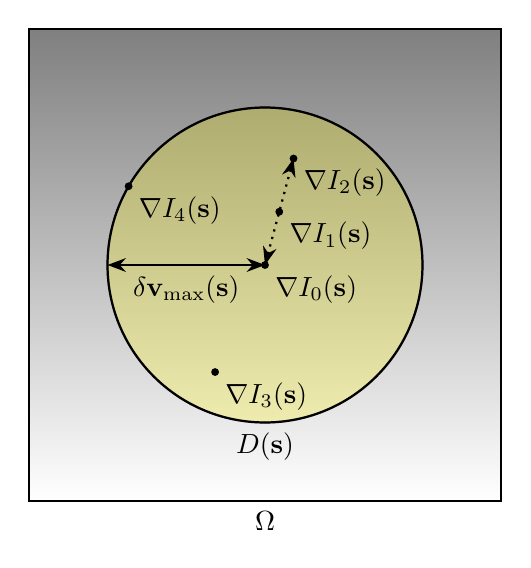
\begin{tikzpicture}[thick]
\shadedraw[] (-3,-3) rectangle (3, 3);
\filldraw[fill=yellow, opacity=0.25] (0, 0) circle (2);
\draw (0, 0) circle (2);
\coordinate[label = below right: $\nabla I_{0}(\mathbf{s})$] (O) at (0,0);
\coordinate[label = below right: $\nabla I_{1}(\mathbf{s})$] (A) at (75:0.7);
\coordinate[label = below right: $\nabla I_{2}(\mathbf{s})$] (B) at (75:1.4);
\coordinate[label = below right: $\nabla I_{3}(\mathbf{s})$] (C) at (245:1.5);
\coordinate[label = below right: $\nabla I_{4}(\mathbf{s})$] (D) at (150:2.0);
\coordinate[label = below:$D(\mathbf{s})$] (Z) at (270:2);
\coordinate[label = below: $\Omega$] (Y) at (270:3);
\coordinate[] (X) at (180:2);
\coordinate[label = below:$\delta \mathbf{v}_{\max}(\mathbf{s})$] (W) at (180:1);
% lets place the dots
\node at (O)[circle,fill,inner sep=1pt]{};
\node at (A)[circle,fill,inner sep=1pt]{};
\node at (B)[circle,fill,inner sep=1pt]{};
\node at (C)[circle,fill,inner sep=1pt]{};
\node at (D)[circle,fill,inner sep=1pt]{};
\draw[Stealth-Stealth] (O) -- (X);
\draw[Stealth-Stealth, dotted] (O) -- (B);
\end{tikzpicture}

\end{document}